\chapter{显示模块}

\section{摄像头介绍}

本系统选用的主要摄像头为熙晟微品牌的18\_U3\_K2MP与18U2\_K2MP型号,尺寸为94×49×54mm,工作电压5V,支持USB3.0和USB2.0两种接口输出。该摄像头最高支持1920×1080(30帧/60帧)以及1280×720(30帧/60帧/120帧)多种分辨率和帧率,像素达200万,广泛应用于无人机、工业产线检测、直播、机器人巡逻等领域。其多帧率切换和自动变焦功能,为系统图像处理与深度学习检测提供稳定可靠的数据源。

为保障系统的性能、兼容性与成本均衡,项目团队调研了市场上主流品牌摄像头产品,包括海康威视(Hikvision)、大华、熙晟微、罗技(Logitech)、DEPSTECH 等,从分辨率(如1080P、4K)、接口类型(USB、以太网POE、WiFi/4G/5G)、编码格式(H.264、MJPEG)、夜视能力、变焦功能以及价格、可开发性多个维度进行了深入对比。表\ref{tab:camera_comparison} 汇总了部分典型摄像头选型信息。

\begin{table}[H]
    \centering
    \caption{摄像头选型对比表}
    \label{tab:camera_comparison}
    \renewcommand{\arraystretch}{1.2} % 可选,增加行高
    \setlength{\tabcolsep}{3pt} % 可选,减少列间距
    \begin{tabular}{|c|c|c|c|c|c|p{4cm}|c|}
        \hline
        序号 & 通信方式 & 电源方式 & 夜视 & 变焦 & 可开发 & 其他 & 价格 \\
        \hline
        1 & WIFI/5G & 插电 & 可选 & 支持 & 否 & 需连接手机APP,不支持二次开发 & 699 \\
        \hline
        2 & WIFI/4G & 插电 & 否 & 否 & 支持 & 多协议,支持开发 & 299 \\
        \hline
        3 & WIFI & 插电 & 支持 & 否 & 支持 & 1080p,带云台,可开发 & 438 \\
        \hline
        4 & ISUP5.0 & 太阳能 & 否 & 否 & 支持 & 防水防尘,支持SDK开发 & 4315 \\
        \hline
        5 & 以太网通信 & 插电 & 支持 & 否 & 支持 & 红光夜视30m,白光20m & 500 \\
        \hline
        6 & USB通信 & 插线 & 否 & 否 & 支持 & 工业相机,适用距离3-5m & 272 \\
        \hline
        7 & USB通信 & 插线 & 否 & 支持 & 支持 & 工业相机,18倍变焦,适用于机器人训练 & 650 \\
        \hline
    \end{tabular}
\end{table}

\section{网页前后端介绍}

本系统采用基于Flask的Python后端与前端网页架构,实现多摄像头视频流的实时监控与管理。后端通过OpenCV负责多路摄像头视频采集与快照缓存,采用多线程实现轮询采集,避免多摄像头资源冲突。系统设计全局快照缓存,非激活摄像头显示最近缓存图像,激活摄像头提供实时视频流,提升用户体验。

主要功能模块包括:

\begin{itemize}[leftmargin=*]
  \item \textbf{摄像头采集线程}:定时轮询各摄像头,采集图像并更新缓存,支持动态添加与切换。
  \item \textbf{视频流生成}:通过HTTP multipart响应,将激活摄像头实时视频流推送至前端,延迟低、流畅度高。
  \item \textbf{接口设计}:提供API接口支持查询当前激活摄像头、切换摄像头、获取快照等功能,前端控制灵活。
  \item \textbf{前端页面}:主页以缩略图形式展示所有摄像头快照,点击进入单摄像头实时视频页面,界面简洁直观。
\end{itemize}

\begin{figure}[H]
    \centering
    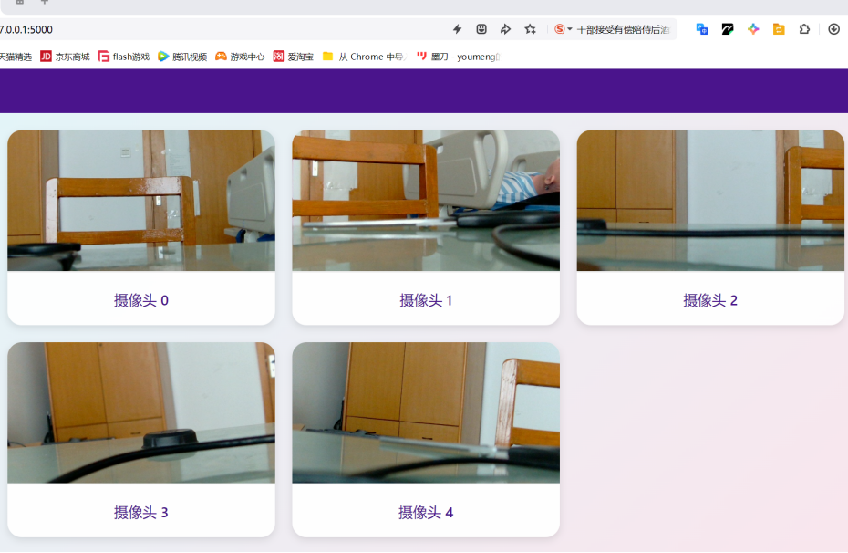
\includegraphics[width=0.85\textwidth]{web_test1.png}
    \caption{系统前端网页界面示例}
    \label{fig:web_test1}
\end{figure}

如图\ref{fig:web_test1}所示,系统前端页面实现了多摄像头缩略图展示及实时切换,界面布局清晰,用户操作直观,适配多种终端浏览器。

\section{洪水数据集收集与整理}

为了支持本项目在灾害识别及预警中的应用,团队对洪水场景图像数据进行了系统化收集与整理,确保后续模型训练具备充分多样的数据支持。主要工作流程如下:

\subsection{数据源调研与筛选}

通过HuggingFace、Google Dataset Search 等平台,搜集国内外公开洪水图像数据集与相关研究资源,重点对比各数据源的图像数量、清晰度、标注信息完整性等关键指标,并筛选出质量较高、可直接用于模型训练与测试的数据集。

此外,特别关注多场景(如城市内涝、河流泛滥、道路积水等)及多视角图像,保证数据的多样性与泛化能力,提升模型对不同类型洪水场景的识别准确率。

\subsection{图像数据收集与管理}

除公开数据集外,利用搜索引擎与公开视频平台,手动筛选下载典型洪水场景图片,并对部分洪水视频,使用工具按帧提取关键图像,以丰富数据集内容。

所有图像按照场景类别、拍摄角度等维度进行分类与统一命名,方便后续的模型训练、验证及人工标注。

\subsection{数据清洗与格式整理}

对收集到的所有图像进行去重,剔除重复、模糊、无效图像,确保数据质量。同时统一图像文件格式(如 PNG / JPG),调整分辨率为网络输入标准,保证模型训练效率。

最终,将整理好的数据集按训练集、验证集、测试集分目录打包,目录结构清晰,如图\ref{fig:dataset_tree}所示。

\begin{figure}[H]
    \centering
    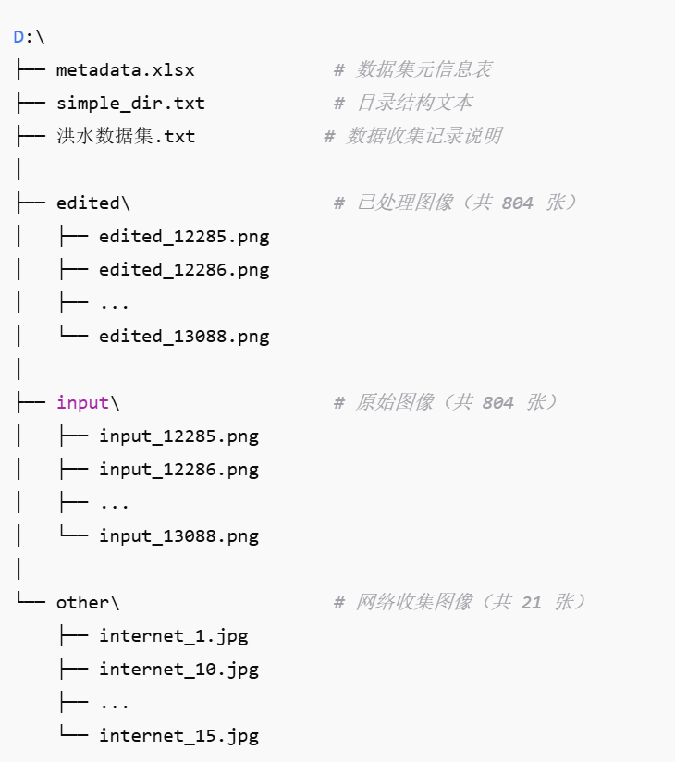
\includegraphics[width=0.6\textwidth]{dataset_tree.png}
    \caption{洪水图像数据集目录结构示例}
    \label{fig:dataset_tree}
\end{figure}

\subsection{工作成效}

通过上述流程,成功构建了一个种类丰富、结构规范的洪水图像数据集,为后续开展洪水场景图像识别、目标检测、场景分类及灾害预警算法研究提供了坚实的数据基础。


\section{改进方向}

\subsection{系统可扩展性}

目前系统监控范围主要受限于摄像头物理安装位置与单台摄像头识别距离(一般为10-20米范围内高质量图像采集)。通过增加摄像头数量与合理布局,可覆盖更大区域,提升监控盲区冗余。同时,利用摄像头自动变焦与深度学习模型识别结果结合,可动态聚焦目标,进一步提升识别精度。

\subsection{网页前后端优化}

\begin{itemize}[leftmargin=*]
  \item 前端引入WebSocket替代HTTP轮询,支持多摄像头实时并发预览,降低延迟,提升交互体验。
  \item 增加摄像头控制面板,支持变焦、旋转、曝光等硬件参数的远程配置。
  \item 后端可升级为异步框架(如FastAPI、Quart)或使用多进程架构,提升处理并发能力。
  \item 结合边缘计算,将部分图像预处理分配至摄像头端或转发服务器,减轻主服务器负载。
  \item 增强安全认证与访问控制,防止未授权访问与潜在的数据篡改风险。
\end{itemize}

\subsection{其他改进建议}

\begin{itemize}[leftmargin=*]
  \item 引入智能告警功能,检测到危险情况自动推送短信、邮件或APP通知,提高响应速度。
  \item 升级图像分割与检测模型,如使用YOLOv8更大版本或SAM模型,提升检测精度与鲁棒性。
  \item 兼容更多摄像头协议,如RTSP、RTMP,拓展设备适配范围。
  \item 增加日志管理与自动故障恢复机制,保障系统稳定性与可维护性。
  \item 优化无线网络架构,采用环形拓扑与多级中继,提升野外复杂环境下的网络可靠性与覆盖范围。
\end{itemize}


